\newpage

\section{Brute force}

\subsection{Description de la vunérabilité}

Une tentative d’attaque de type brute force intervient, pour une application web, au niveau de l’interface login. Le but de cette attaque est de se connecter en essayant plusieurs combinaisons login / mot de passe jusqu’à arriver à une combinaison acceptée par le système. Il est à supposer ici qu’un nombre infini de tentative est possible.

L’attaque de type Force Brute peut se faire de deux manières différentes : avec ou sans dictionnaire. 

Dans le cas d’une attaque sans dictionnaire, pour chaque login connu, il faut tenter toutes les combinaisons d’un ou plusieurs caractères alphanumériques jusqu’à correspondance avec le login choisi.
Pour une attaque avec dictionnaire, il faut créer un fichier contenant par exemple les mots de passe les plus souvent utilisés. Pour chaque login connu, chaque mot de passe contenu dans le fichier créé sera testé, en espérant qu’au moins un parmi la liste corresponde.

Une telle attaque peut être un premier point d’appui pour obtenir plus de privilèges sur l’application web. De plus, si une personne utilise souvent le même mot de passe, l’attaquant pourra le réutiliser sur d’autres applications comme les réseaux sociaux.


\subsection{Exploitation de la vulnérabilité}

On se place dans l’onglet Brute Force. On retrouve un espace avec deux champs à remplir : le login (username) et le mot de passe (password) associé. Il est possible de tenter de se loger en essayant plusieurs combinaisons parmi les plus courantes telles que : 'root, root', `admin, admin', `administrateur, password'… On trouvera assez rapidement une combinaison login / mot de passe qui convient.

L’autre méthode s’appuie sur un dictionnaire. On crée donc un fichier, que l’on nomme 'motsdepasse.txt', contenant les mots de passe les plus utilisés. Il est aussi possible d’y rajouter des informations sur les utilisateurs (ville de résidence, noms des enfants, année de naissance, …) pour étendre l’éventail de recherche des combinaisons login / mot de passe.

Après le premier essai, on remarque que les champs login et mot de passe interviennent dans l’URL. http://localhost/dvwa/vulnerabilities/brute/?username=admin&password=password&Login=Login#. Les essais à répétition se feront donc sur l’URL en remplaçant les champs username et password par un login choisi au préalable, et un mot de passe parmi la liste du fichier de mots de passe créé précédemment.

Après l’attaque, on remarque que la combinaison username = admin, password = password est censé fonctionner. Il est possible de vérifier en rentrant ces données dans les champs concerné.


On arrive bien à se connecter au système en tant qu’admin :

\begin{figure}[!h]
\begin{center}

\label{inclusion}
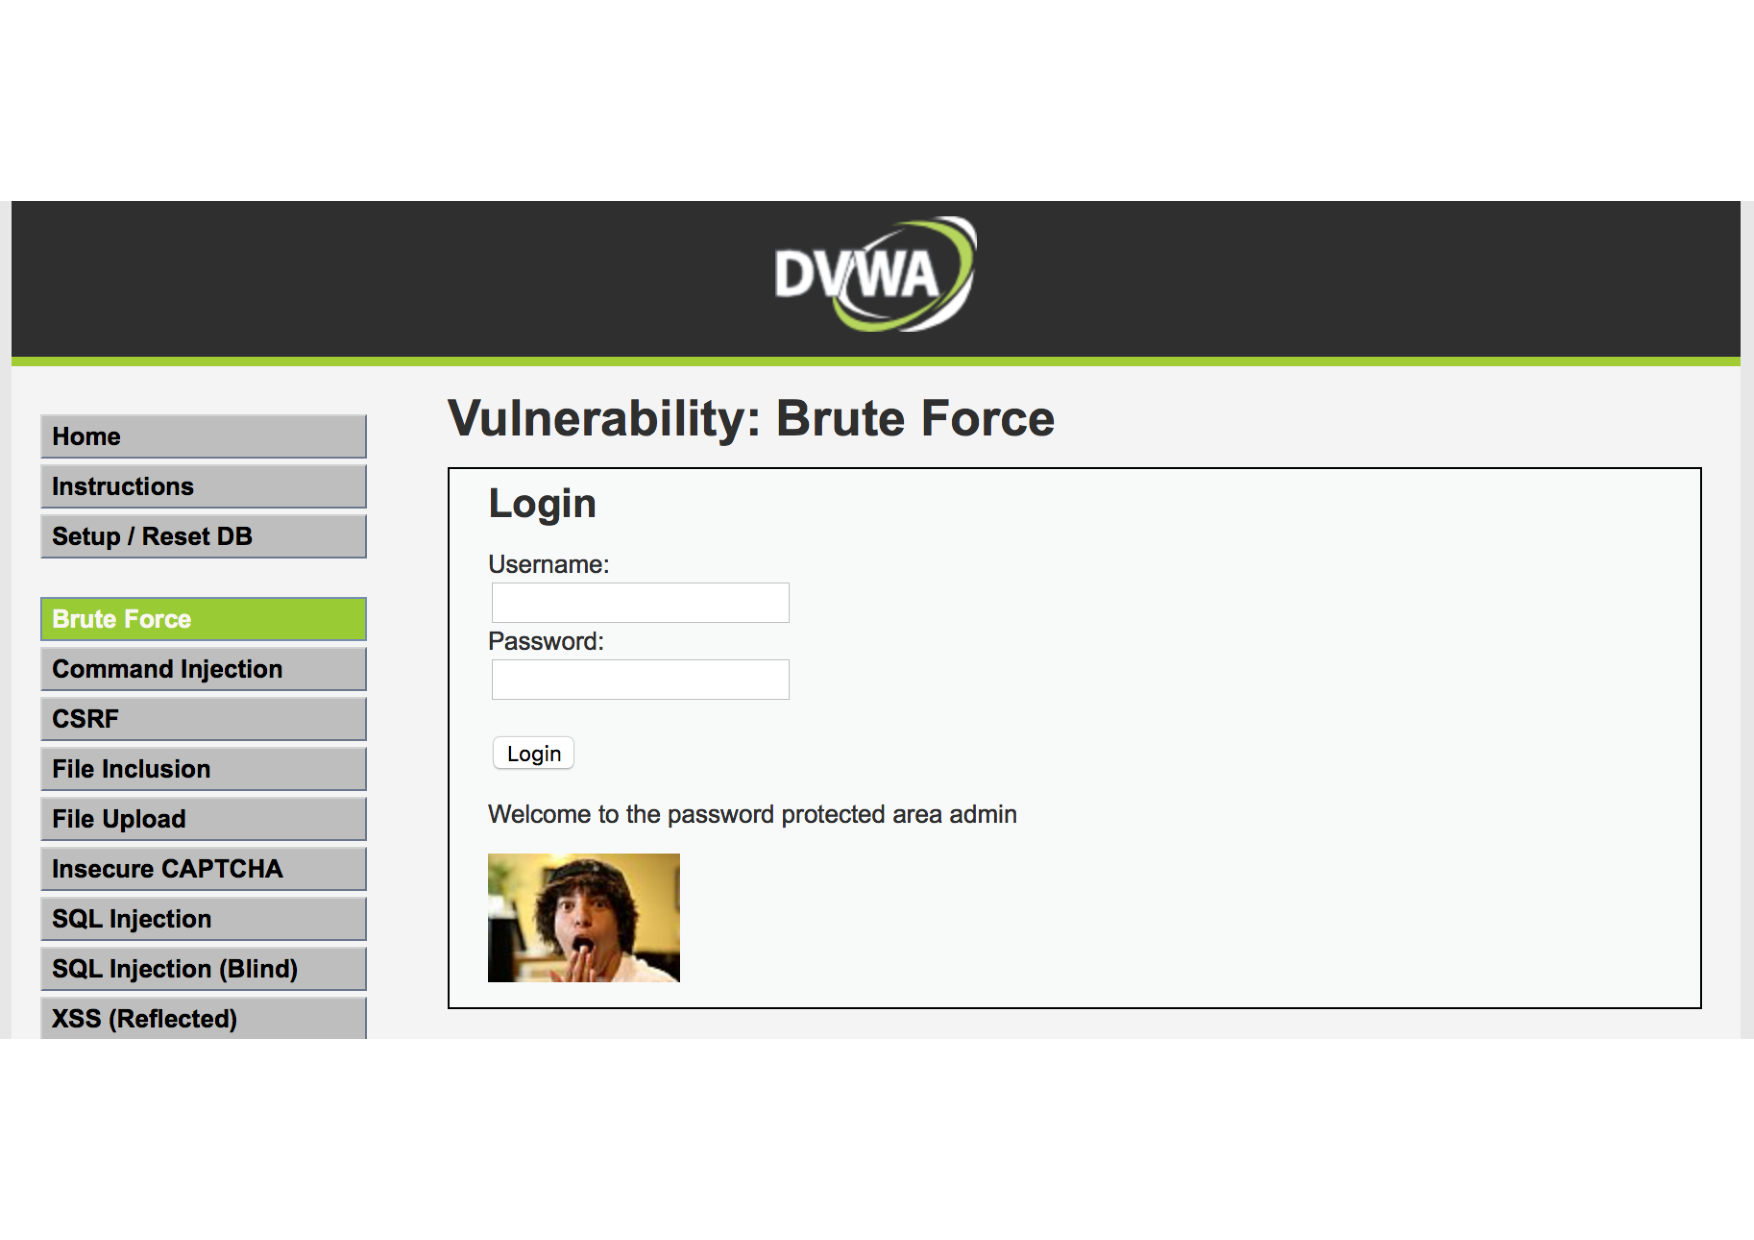
\includegraphics[scale=1.2]{images/BruteForce-ConnexionAdmin.pdf}

\caption{Brute Force - Connexion admin}

\end{center}
\end{figure}

\subsection{Contre-mesure}

Afin de protéger l’application contre une attaque de type Brute Force, plusieurs méthodes se présentent à nous.

Tout d’abord, le mot de passe qui est utilisé ici peut être qualifié de faible. En effet le mot de passe 'password' n’est pas assez complexe pour sécuriser le compte admin. Il faut donc utiliser des mots de passe ne faisant pas partie des plus utilisés, mais aussi respectant des règles telles que :
\begin{enumerate}
\item Au moins 8 caractères;
\item Au moins un caractère spécial (#, @, …);
\item Au moins un caractère numérique;
\item Au moins un caractère majuscule et minuscule;
\item …
\end{enumerate}

Ensuite, il était possible d’effectuer un nombre infini d’essai de mot de passe pour un login donné. Il serait intéressant de mettre un place un système de comptage d’essai, et de limiter ce nombre d’essai, à trois par exemple. Suite à ces trois essais, le compte serait bloqué.

Une autre donnée à laquelle nous avions accès était le login connu par avance. Afin de palier à ce problème, le login peut être affichier d'une manière différente lorsque l'utilisateur est déja logé.

Enfin, une dernière méthode pourrait être d'effectuer la connexion par le moyen d'une entrée qui ne peut être attaquée grâce a la Brute Force telle que des empreintes personnelles ou encore une signature.

\section{Command injection}

\subsection{Description de la vulnérabilité}

Une tentative d’attaque par exécution de commandes consiste, comme son nom l’indique, à exécuter des commandes à partir d’un champ d’une application web. L’intérêt est ici de pouvoir exécuter ces commandes dans le serveur web. Il est à savoir que les commandes lancées dans ce serveur le sont avec les droits du serveur.

Ce type d’attaque peut servir de premier point d’entrée pour une attaque de plus grande ampleur dans l’application web visée.


\subsection{Exploitation de la vulnérabilité}

On se place dans l’onglet Command Execution. Ici on doit rentrer une adresse IP pour effectuer un ping vers cette adresse. On peut tester ce ping en entrant 'localhost' :

\begin{figure}[!h]
\begin{center}

\label{inclusion}
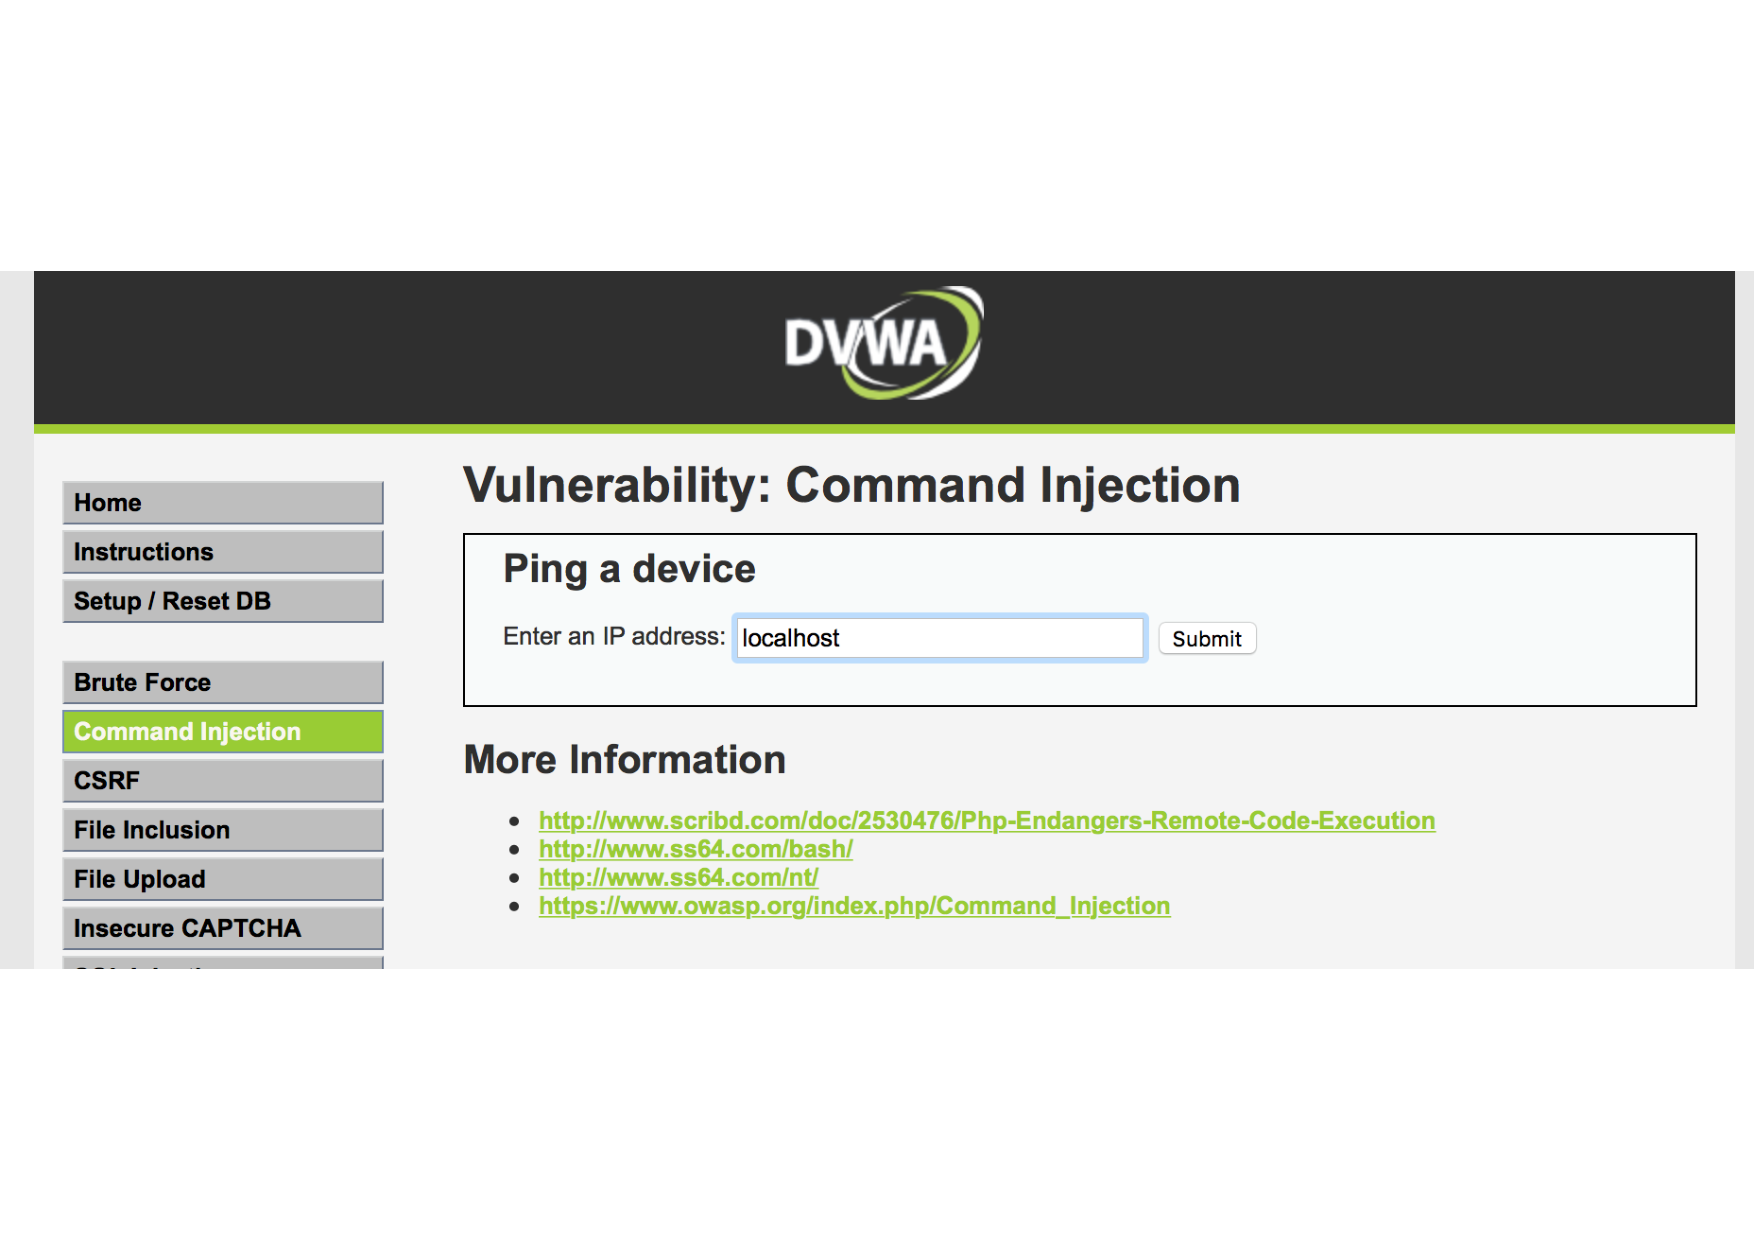
\includegraphics[scale=1.2]{images/CommandInjection-Localhost.pdf}

\caption{Command Injection - Localhost}

\end{center}
\end{figure}

Ce qui donne :

\begin{figure}[!h]
\begin{center}

\label{inclusion}
\includegraphics[scale=1.2]{images/CommandInjection-LocalhostRésultat.pdf}

\caption{Command Injection - Localhost résultat}

\end{center}
\end{figure}

On peut essayer de rentrer une commande après l’adresse choisie en séparant celles-ci d’un ';'. Par exemple, en rentrant la commande 'localhost ; ls', on obtient :

\begin{figure}[!h]
\begin{center}

\label{inclusion}
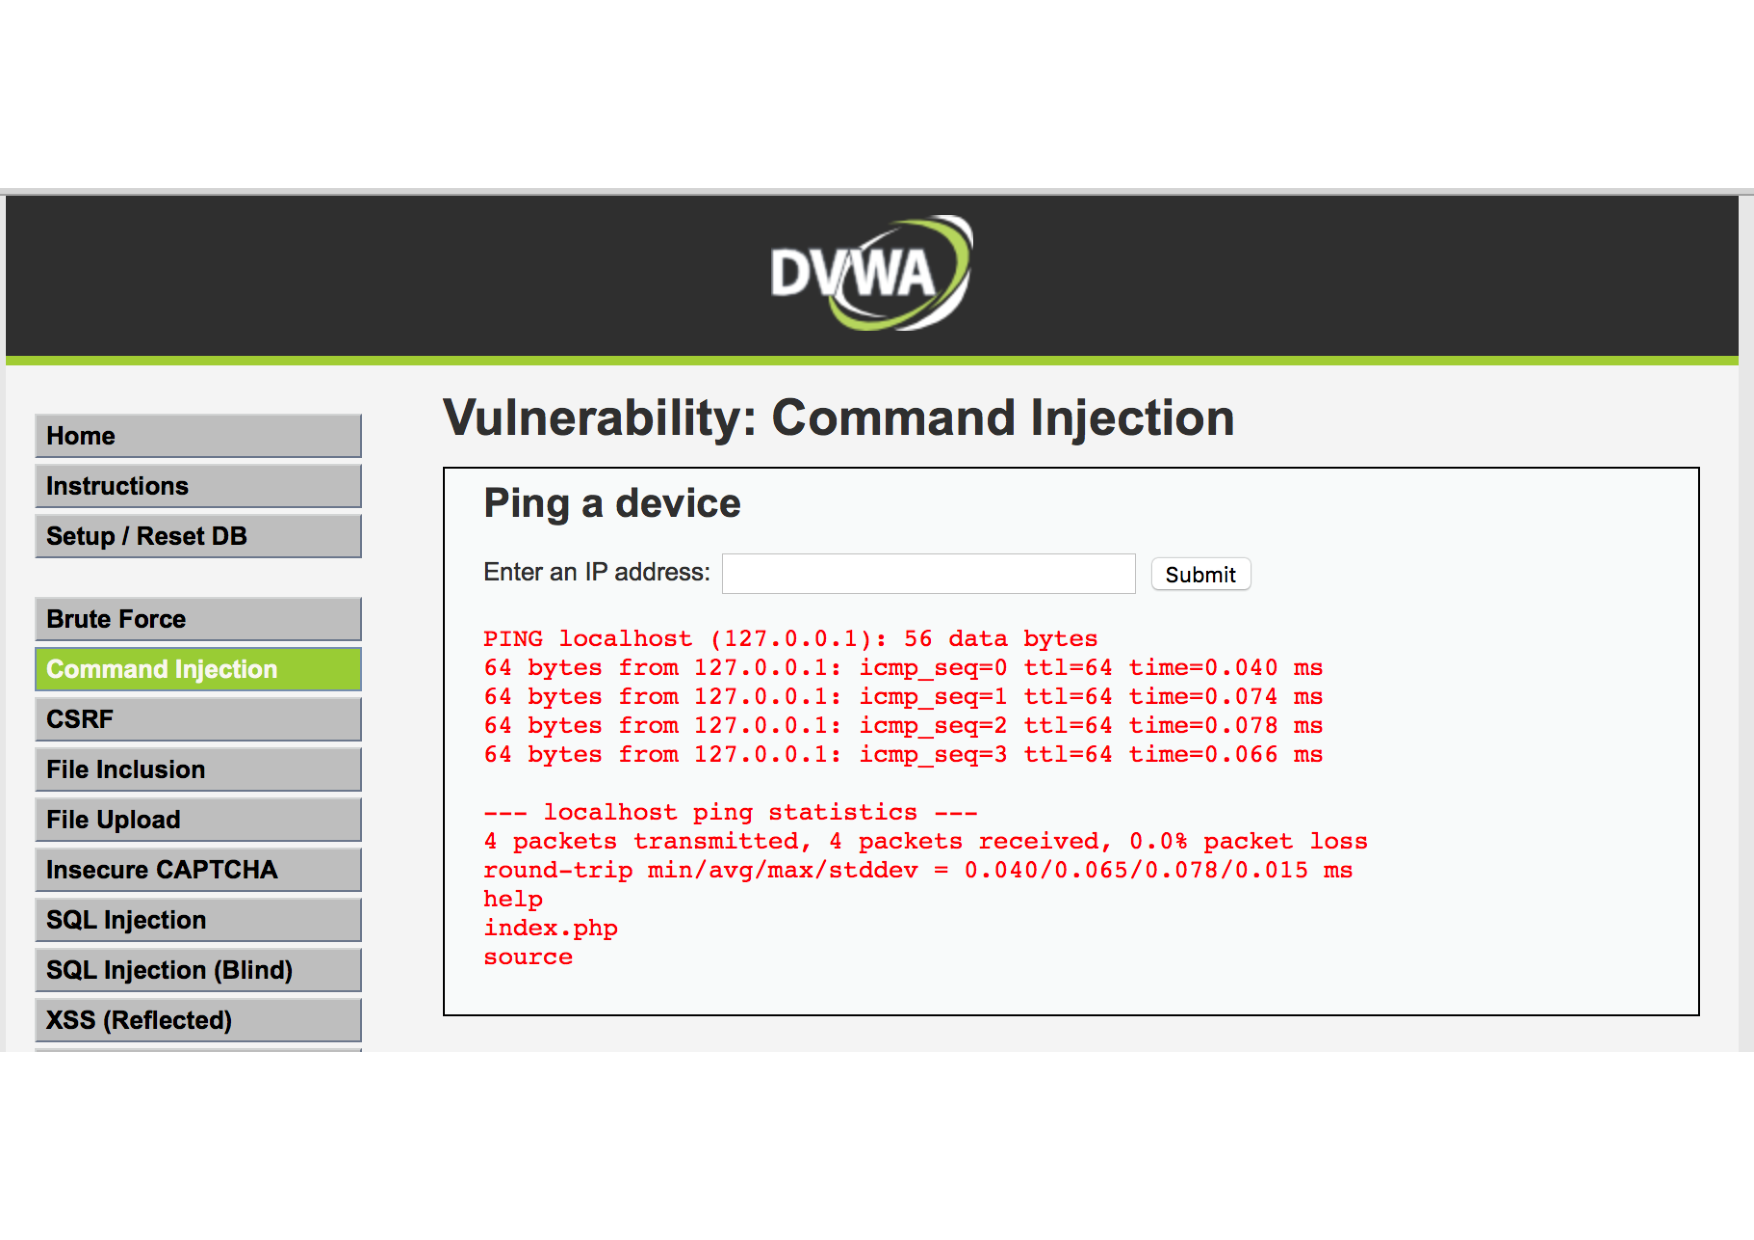
\includegraphics[scale=1.2]{images/CommandInjection-Localhost;ls.pdf}

\caption{Command Injection - Localhost ; ls}

\end{center}
\end{figure}

On a donc un listing de l’ensemble des fichiers et des répertoires présents dans le répertoire où l’on se trouve.
Il devient alors possible de lancer des commandes à partir de cette barre de recherche. De plus, il est possible d’enchaîner les commandes en les séparant par ';' et donc de naviguer dans les répertoires du système.


\subsection{Contre-mesure}


\section{ CSRF}

\subsection{Description de la vulnérabilité}

Une attaque de type CSRF, Cross-Site Request Forgery, consiste à faire agir un utilisateur, comme on le désire, à son insu. L'objectif principal est de générer une action particulière. Ces actions peuvent être de plusieurs types :

\begin{enumerate}
\item créer, supprimer ou modifier un utilisateur;
\item changer de mot de passe;
\item créer, supprimer ou modifier un article sur une page web;
\item modifier les options d'une application web;
\item …
\end{enumerate}


\subsection{Exploitation de la vulnérabilité}

\subsection{Contre-mesure}

Afin de prévenir une application web de ce type d'attaque, certaines protections peuvent être mises en place.

Premièrement, lorsque l'action est sur le point d'être effectuée, une confirmation ou encore une authentification supplémentaire pourrait être demandée pour valider l'action.Pour que cela soit efficace, il faut encore que le mot de passe et le login ne soient pas connus par l'attaquant.

Pour renforcer la protection contre cette attaque, une etape efficace est de se deconnecter avant de quitter une application web. De cette manière, les cookies sont désactivés définitivements et sont supprimés.

Certaines applications web peuvent demander aux utilisateurs s'il désirent enregistrer leur login et leur mot de passe. Afin de ne pas s'exposer à une attaque de type CSRF, il est déconseiller d'enregistrer le mot de passe pour la connexion d'un utilisateur.

Enfin, il peut être intéressant d'utiliser plusieurs navigateurs pour séparer les utilisations personnelles des utilisations standards d'applications web. Cela permettra de rendre impuissante l'utilisation d'une attaque d'un telle type.




